

\documentclass{article}
\usepackage[utf8]{inputenc}
\usepackage{setspace}
\usepackage{ mathrsfs }
\usepackage{graphicx}
\usepackage{amssymb} %maths
\usepackage{amsmath} %maths
\usepackage[margin=0.2in]{geometry}
\usepackage{graphicx}
\usepackage{ulem}
\setlength{\parindent}{0pt}
\setlength{\parskip}{10pt}
\usepackage{hyperref}
\usepackage[autostyle]{csquotes}

\usepackage{cancel}
\renewcommand{\i}{\textit}
\renewcommand{\b}{\textbf}
\newcommand{\q}{\enquote}
%\vskip1.0in





\begin{document}

{\setstretch{0.0}{
Cesium [ Julia Version ]

Cesium is a highly adjustable symmetric cryptosystem that uses an $n \times n$  matrix of integers in $1..b$ as a key, with $b$ and $n$ chosen by the user. Larger values of $b$ and $n$ should be more secure. It's also easy to let $n =b$, but this is not required (or desired, if $b$ is small.)

Cesium is a mutation of Cyclone. In Cyclone, each row had to represent a permutation. In Cesium, this constraint is lifted. Indeed there are no constraints, though choosing a matrix of all $7$s, for instance, would not be great for security, given how the key is used.

The diagonal of the matrix does the work here. Let's look at the crucial functions:


\begin{verbatim}
function encode(p,q)
    k = copy(q)
    c = Int64[]
    for i in eachindex(p)
        x = tr(k)%b
        push!(c,(p[i] + x)%b )
        isodd((x + p[i])%b) ? spincols(k,p[i]) : spinrows(k,p[i])
    end
    c
end


function spinrows(k,p)
    for j in 1:size(k)[begin]
            k[j,:] = circshift(k[j,:],k[j,j]+p + 1)
    end
end


function spincols(k,p)
    for j in 1:size(k)[begin]
        k[:,j] = circshift(k[:,j],k[j,j]+ p + 1)
    end 
end

\end{verbatim}

The next cipher symbol is the sum of the trace of the key matrix and the plain symbol (mod $b$, so that $c \in 1..b$). Then each row is circular-shifted by $p + 1$ units, so that the key's evolution is strongly dependent on the plaintext (which should add security.) 
 

An adjustable \q{alphabetic mask} is also used for a more human-readable output. For instance, we can set $n = 26$ and then translate representations of the key, plaintexts, and ciphertexts by $1 \to a, 2 \to b,3 \to c,...$. The images below show outputs from the demo function.



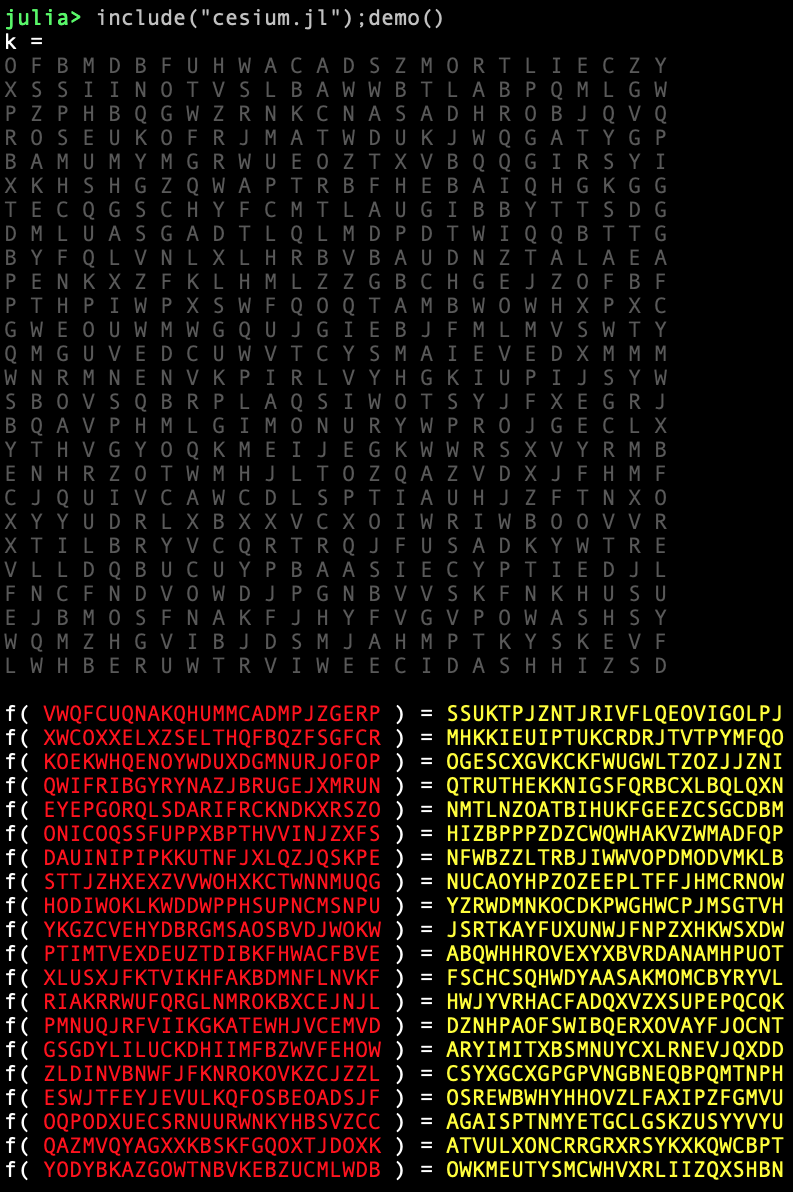
\includegraphics[width=0.5\textwidth]{1.png}
\begin{figure}[h!]
\end{figure}




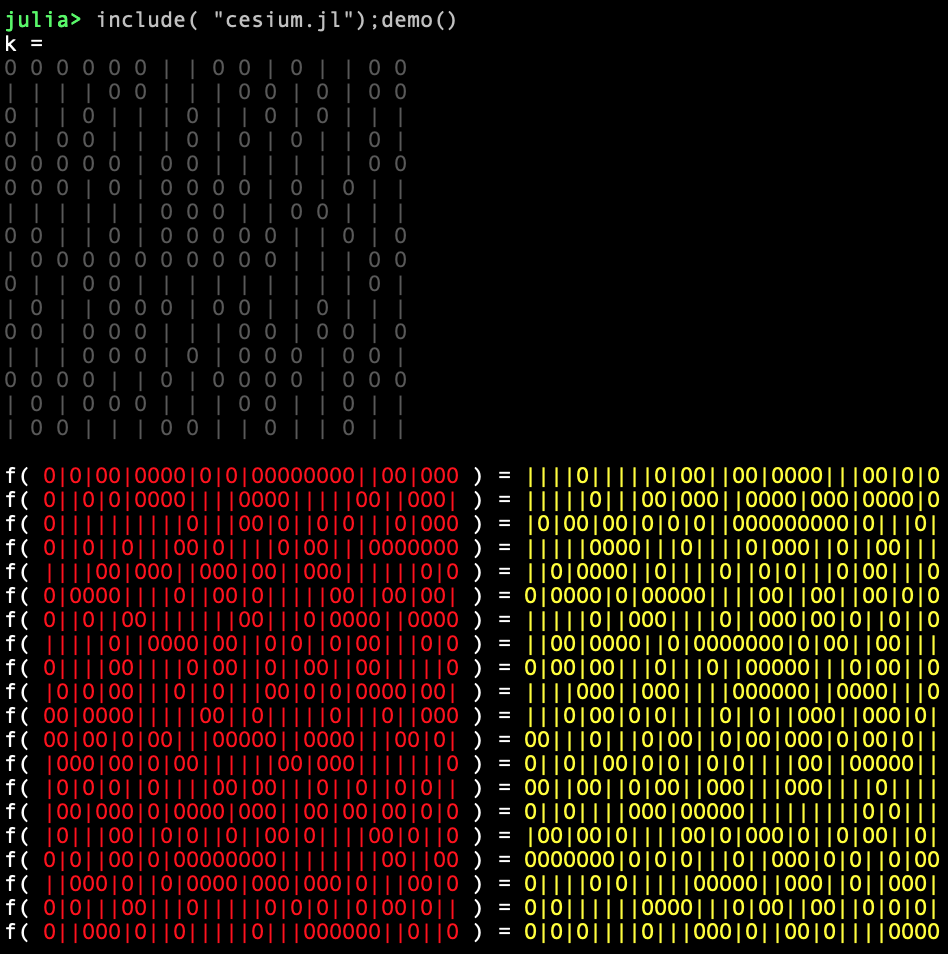
\includegraphics[width=0.5\textwidth]{2.png}
\begin{figure}[h!]
\end{figure}

The second image could also be of the Thorium cryptosystem, which is basically the Cesium system with $b = 2$. I hope to write Thorium so that its bit-centric nature is emphasized. Curium is another variant, where $b = 3$ and the $27$ symbols of the alphabet and (for instance) the underscore are encoded in three ternary digits, so that plaintext messages in English are translated into ternary and then encoded. 



}}
\end{document}
